% Template for IWAENC 2012 paper; to be used with:
%          spconf.sty  - ICASSP/ICIP LaTeX style file, and
%          IEEEbib.bst - IEEE bibliography style file.
% --------------------------------------------------------------------------
\documentclass{article}
\usepackage{spconfa4,amsmath,graphicx}
\usepackage{epsf,psfig}
\usepackage{epstopdf}
\usepackage[noadjust]{cite}
\usepackage{filecontents}
\usepackage{subfigure}
\usepackage[export]{adjustbox}
% Title.
% ------
\title{Design of Robust Differential Microphone Arrays of Arbitrary Geometry}
%
% Single address.
% ---------------
\name{Itay Yehezkel Karo, Yaakov Buchris and Israel Cohen}%\thanks{Thanks to XYZ agency for funding.}}
\address{} %{Author Affiliation(s)}
%
% For example:
% ------------
%\address{School\\
%	Department\\
%	Address}
%
% Two addresses (uncomment and modify for two-address case).
% ----------------------------------------------------------
%\twoauthors
%  {A. Author-one, B. Author-two\sthanks{Thanks to XYZ agency for funding.}}
%	{School A-B\\
%	Department A-B\\
%	Address A-B}
%  {C. Author-three, D. Author-four\sthanks{The fourth author performed the work
%	while at ...}}
%	{School C-D\\
%	Department C-D\\
%	Address C-D}
%
\begin{document}
%\ninept
%
\maketitle
%
\begin{abstract}
%Many articles about differential microphone arrays and general arrays handle the trivial case of the linear or circular arrays when developing their equations. In This article we present an expansion for the article ''Design of Robust Differential Microphone Arrays'' \cite{sps17} that deals with the option of gaining robustness by processing an array with lower order than the number of elements in the array. We free ourselves from the linear array assumption and manipulate the system proposed in the article to our general case. We will present simulations of various geometries and see their effect on the final result in terms of directivity gain and white noise gain.
Differential microphone arrays (DMAs) can be used for several applications including speech signals processing. Their main contribution is to process broadband signals and reconstruct them with higher signal-to-noise ratio. Even though DMAs are characterized as super-directive former, they suffer from the problem of high white noise amplification, especially in low frequencies. One of the approaches to handle the white noise amplification problem was recently proposed. This approach use more microphones than the minimal required and based on the Maclauren's series approximation' design a robust version of the DMAs for linear geometry. In this paper, we generalized this approach for any arbitrary geometry. 
\end{abstract}
%
\begin{keywords}
Array processing, wide-band, pattern, forming, Differential microphone arrays (\textbf{DMAs}), directivity factor, white noise gain, arbitrary geometry.
\end{keywords}
%
\section{Introduction}
\label{sec:intro}
In some real-world audio applications, such as hands-free telecommunication, environment effects like background noise and reverberation, may degrade the quality of speech signals.
Speech enhancement methods that are based on microphone arrays have been of important research interest for several decades \cite{sps1,sps3,sps4}. 
Among these methods, differential microphone arrays (DMAs), which enable wide-band frequency invariant beampatterning, have shown their great potential recently  \cite{sps6,sps7}. 
As early as in the 1940s, differential microphone arrays (DMAs) of different orders were constructed and their anti-noise characteristics were analyzed. Since then, a good amount of progress has been made. 
In \cite{sps10,sps11}, adaptive DMAs were developed to suppress spatially non-stationary noise. 
In \cite{sps14,sps15}, approaches for the design of higher-order DMAs were developed.
Though a conventional $ N $th-order DMA, which consists of $ N+1 $ microphones, can achieve a high directional gain (i.e., a large SNR gain in diffuse noise), it suffers from poor white noise amplification especially as the order increases \cite{sps6}.
It was suggested in \cite{sps6} and thoroughly studied in \cite{sps17}  
that by using more microphones $ M $ than the order $ N $, we can achieve better robustness to the white noise.
All the references above, have studied the linear array case, a fact that created the motivation for this paper that is actually a continuation of \cite{sps17} and generalization of the study to an arbitrary geometry array where each microphone can be placed randomly on a 2D plane (with some limitations regarding the wave-length). The silver-lining between  \cite{sps17} and this paper, is coefficient-wise matching between a mathematical beampattern and a Maclauren approximation of the actual array beampattern.
%We have organized the paper as follows. In Section II, the signal model, the formulation of the problem, and some useful definitions are presented. In Section III, the beam pattern and its frequency-independent form are described. Simulations are carried out in Section VII, followed by conclusions in Section VIII.

\section{Problem formulation}
\label{sec:Problem_formulation}

We consider a far-field source signal $ X(\omega) $, that propagates in an anechoic environment at the speed of sound, i.e. $ c=340 \mathrm{[m/s]} $, and impinges on an arbitrary 2D geometry array of sensors consisting of $ M $ microphones. 
The location of each microphone is defined by the pair $ \left(r_m,\phi_m\right) $, where $ r_m $ is the radius and $ \phi_m $ is the angle with respect to an arbitrary point.
The propagation angle $ \theta $ of the source signal and the steering angle $ \theta_s $ are also measured with respect to the same reference point (Fig. \ref{FigLbl_ArrShape}).
\begin{figure}[h]
	% trim={<left> <lower> <right> <upper>}
	\centerline{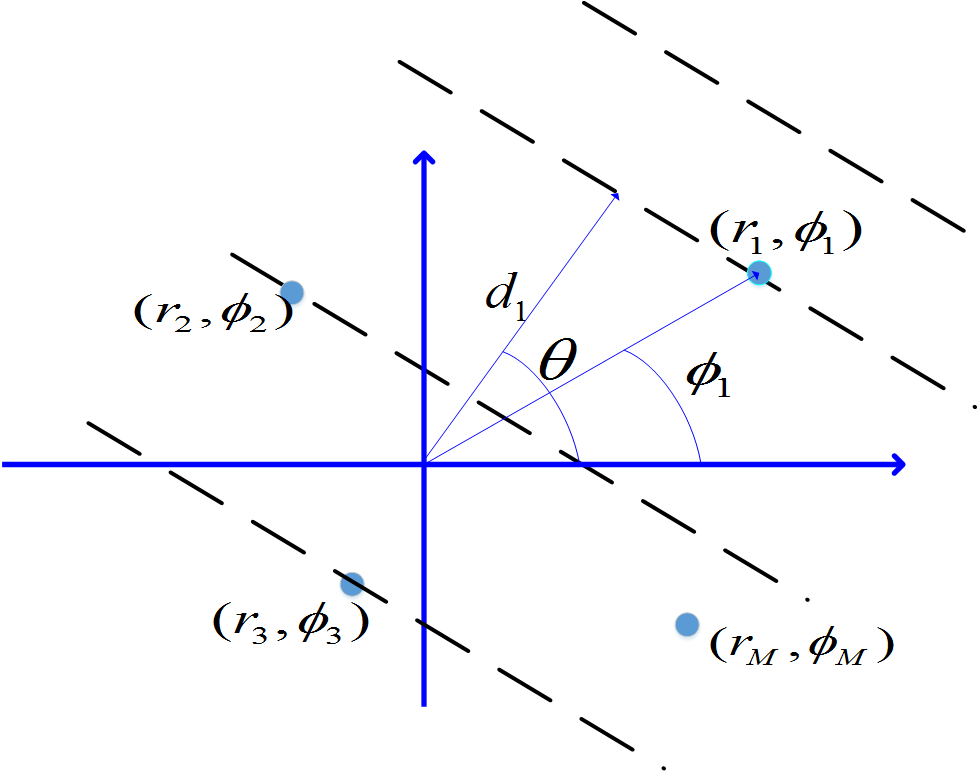
\includegraphics[width=75mm,trim={2cm 2cm 2cm 4cm},clip]{ProblemFormulationVisio.png}} \caption{An arbitrary geometry 2D sensor array.}\label{FigLbl_ArrShape}
\end{figure}\\
The steering vector is defined as
\begin{equation}
\begin{split}
\boldsymbol{d}(\omega,\theta)&=\left[e^{-j\tau_1\omega},e^{-j\tau_2\omega},...,e^{-j\tau_M\omega}\right]^T
\\        \tau_m&=\frac{r_m}{c}\cos{\left(\theta-\theta_s-\phi_m\right)},
\end{split}
\end{equation}
where the superscript $ ^T $ is the transpose operator, 
$ \omega=2\pi f $ is the angular frequency, $ f>0 $ is the temporal frequency, and $ \tau_m $ is the propagation time between the reference point and the m'th sensor.
In DMAs \cite{sps17}, it is always assumed that the sensor spacing $ d_{ij} $ is much smaller than the signal wavelength i.e. $ \omega_{max}{(d_{ij})} << 2\pi \ \forall i,j \in \ \{1..m\} $. The final goal is to methodically construct a set of filters, each receives the data of a single sensor, that by summing their outputs the desired beampattern emerges. The filters vector is denoted as 
\begin{equation}
\boldsymbol{h}(\omega)=\left[H_1(\omega),H_2(\omega),...,H_m(\omega)\right]^T,
\end{equation}
where each filter's input is
\begin{equation}
Y_m(\omega)=e^{-j\tau_m\omega}X(\omega)+V_m(\omega)
\end{equation}
and $ V_m(\omega) $ is the additive noise in the m'th sensor. It is assumed that the desired signal is not correlated with the additive noise. In a vector form, one can write
\begin{equation}
\begin{split}
\boldsymbol{y}_m(\omega,\theta)=&\left[Y_1(\omega),Y_2(\omega),...,Y_M(\omega)\right]^T 
\\
=& \ \boldsymbol{d}(\omega,\theta)X(\omega)+\boldsymbol{v}(\omega),
\end{split}
\end{equation}
and by summing the filters outputs we get
\begin{equation}
\begin{split}
Z(\omega)&=\sum_{m=1}^{M}{H_m^*(\omega)\boldsymbol{y}_m(\omega)}
\\ & =\boldsymbol{h}^H(\omega)\boldsymbol{y}(\omega,\theta)
\\ & =\boldsymbol{h}^H(\omega)\boldsymbol{d}(\omega,\theta)X(\omega)+\boldsymbol{h}^H(\omega)\boldsymbol{v}(\omega)
\end{split}
\end{equation}
where $ Z(\omega) $ is the estimation of the desired signal, $ X(\omega) $ and the superscript $ ^H $ is the conjugate-transpose operator. %For array performance assessment the two main tools \cite{sps17}, diffuse noise gain and the white noise gain, are used. According to \cite{sps21}, the gains for a general planar array are
We conclude this section with definitions of two important performance measures widely used for assessing array designs \cite{sps17}. The first one is  the white noise gain (WNG) which is defined as  
\begin{equation}
{\cal G}_{wn}\left[\boldsymbol{h}(\omega)\right]=\frac{oSNR}{iSNR}=\frac{\left|\boldsymbol{h}^H(\omega)\boldsymbol{d}(\omega)\right|^2}{\boldsymbol{h}^H(\omega)\boldsymbol{h}(\omega)}
\end{equation}
and the second is the directivity factor (DF) 
\begin{equation}
{\cal G}_{dn}\left[\boldsymbol{h}(\omega)\right]=\frac{\left|\boldsymbol{h}^H(\omega)\boldsymbol{d}(\omega)\right|^2}{\boldsymbol{h}^H(\omega)\boldsymbol{\Gamma}_{dn}(\omega)\boldsymbol{h}(\omega)},	
\end{equation}
where 
\begin{equation}
[\boldsymbol{\Gamma}_{dn}(\omega)]_{ij}=\frac{\sin{[\omega\tau_{ij}]}}{\omega\tau_{ij}}=sinc\left[\omega\tau_{ij}\right]
\end{equation}

and  $ \tau_{ij} $ is the propagation time between sensors $ i $ and $ j $. %, the white noise gain measures the input-to-output SNR improvement in the presence of white noise and the diffuse noise gain measures the same improvement but in case that equal energy noise is coming from all directions \cite{sps17}.

\section{Beam-Patterns}
\label{sec:Beam-Patterns}
The beam pattern of an array specifies its spatial gain to signals with respect to their angle of propagation. Designing beampatterns means adjusting the pattern to meat some constrains that are dictated by the application. 
%In \cite{sps6,sps7} the beam pattern for DMAs is described as a series of cosines 
%\begin{equation}\label{EqLbl_BasicBp}
%	B_{D,N}(\theta)=\sum_{n=0}^{N}a_n\cos^n{(\theta-\theta_s)}.
%\end{equation}
%%where $ \theta_s $ is the steering angle of the array. 
%I linear geometry arrays $ \phi_m=0 \ \forall m \in {1..M} $, which results in
%\begin{equation}
%	\begin{split}
%		& d\left(\theta,\omega\right)=\left[e^{-j\tau_1\omega t},...,e^{-j\tau_M\omega t}\right]^T \\& =\left[e^{-j\frac{r_1}{c}\cos{(\theta-\theta_s)}\omega t},...,e^{-j\frac{r_M}{c}\cos{(\theta-\theta_s)}\omega t}\right]^T.
%	\end{split}
%\end{equation}
%By using the Maclaurin’s series
%\begin{equation}\label{EqLbl_MaclaurenSer}
%	e^x=\sum_{n=0}^{\infty}\frac{1}{n!}x^n
%\end{equation}
%we get 
%\begin{equation}
%	\begin{split}
%		d(\theta,\omega)=\bigg[&{\sum_{n=-\infty}^{\infty}}c_{1n}\cos^n{(\theta-\theta_s)},\sum_{n=-\infty}^{\infty}c_{2n}\cos^n{(\theta-\theta_s)},\\
%		&...,\sum_{n=-\infty}^{\infty}c_{Mn}\cos^n{(\theta-\theta_s)}\bigg]^T		
%	\end{split}
%\end{equation}
The fundamental idea of designing the beampatterns in \cite{sps17} is elementwise matching between the coefficients of the desired mathematical beam pattern 
\begin{equation}
{\cal B}_{D,N}(\theta)=\sum_{n=0}^{N}\alpha_n\cos^n{\theta}+\beta_n\sin^n{\theta} 
\end{equation} 
and those of the practical beampattern of the array ($ {\cal B}_M(\theta) $). The matching results in finding the filters that should be assigned to the array sensors. We start by simply presenting the known \cite{sps15} beam pattern of the second order super-cardioid 
\begin{equation}
{\cal B}_{D,2}=0.103+0.484\cos{\theta}+0.413\cos^2{\theta},
\end{equation} 
that will serve as the desired beampattern. Obviously, our main goal is expressing the practical beampattern (actual array output) as a series of sinusoids so that we can match the coefficients. We start by writing the arbitrary geometry steering vector 
\begin{center}
	\begin{equation}\label{EqLbl_ArbGeoSteeringVec}
		\begin{split}
			d(\theta,\omega)=&\left[e^{-j\tau_2\omega t},e^{-j\tau_M\omega t},...,e^{-j\tau_1\omega t} \right] \\ %\resizebox{0.95\columnwidth}{!}{$\displaystyle
			=&\ [e^{-j\frac{r_1}{c}\cos{(\theta-\theta_s-\phi_1)}\omega t} ,e^{-j\frac{r_2}{c}\cos{(\theta-\theta_s-\phi_2)}\omega t},
			\\&...,e^{-j\frac{r_M}{c}\cos{(\theta-\theta_s-\phi_M)}\omega t}]. %$}
		\end{split}
	\end{equation}
\end{center}
Without loosing the generality, we set $ \theta_s=0 $ for convenience. Plugging in (\ref{EqLbl_ArbGeoSteeringVec}) the identity
\begin{equation}
	\cos(\alpha-\beta)=\cos(\alpha)\cos(\beta)+\sin(\alpha)\sin(\beta)
\end{equation}
and combining it with the binomial identity 
\begin{equation}\label{EqLbl_BinomDef}
	(\alpha+\beta)^N=\sum_{n=0}^{N}{\binom{n}{k}\alpha^{n}\beta^{N-n}},
\end{equation}
we get
\begin{equation}\label{EqLbl_SteerVecExp}
	\begin{split}
		& e^{-j\omega\tau_m}=\sum_{n=0}^{\infty}\frac{1}{n!}(-j\omega\tau_m)^n\approx\sum_{n=0}^{N}\frac{1}{n!}(-j\omega\tau_m)^n\\
		& 
		=\sum_{n=0}^{N}\frac{1}{n!}(-j\omega)^n(\frac{r_m}{c})^n\cos^n{(\theta-\phi_m)}\\
		& %=\sum_{n=0}^{N}\frac{1}{n!}(-j\omega)^n(\frac{r_m}{c})^n\sum_{k=0}^{n}\beta_{nk},	
		=\sum_{n=0}^{N}\sum_{k=0}^{n}\sum_{m=1}^{M}\beta_{nkm}H_m(\omega)\cos^k{\theta}\sin^{n-k}{\theta}
	\end{split}
\end{equation}
where 
\begin{equation}\label{EqLbl_BetankDef}
	%\resizebox{0.95\columnwidth}{!}{$\displaystyle \beta_{nk}=\binom{n}{k}\cos^k(\theta-\theta_s)\cos^k(\phi_m)\sin^{n-k}(\theta-\theta_s)\sin^{n-k}(\phi_m)$}.
	\beta_{nkm}(\omega)=\frac{\binom{n}{k}\left(\frac{-j\omega r_m}{c}\right)^n}{n!}\cos^k(\phi_m)\sin^{n-k}(\phi_m).
\end{equation}
We then continue by expanding the general mathematical beampattern $ {\cal B}_{D,N} $ to a more convenient shape,
\begin{equation}
{\cal B}_{D,N}(\theta)=\sum_{n=0}^{N}\sum_{k=0}^{n}\alpha_{nk}\cos^k{\theta}\sin^{n-k}{\theta},
\end{equation} 
which can obviously be degenerated back to the former form (by choosing $ \alpha_{nk}=0 \ \forall \ 0<k<n $). Matching the coefficients between the two beampatterns results in 
\[\resizebox{0.95\columnwidth}{!}{$\displaystyle
	\begin{bmatrix}
	\beta_{001}(\omega) 	& \dots 		& \beta_{00M}(\omega)\\
	\beta_{101}(\omega) 	& \dots 		& \beta_{10M}(\omega)\\
	\beta_{111}(\omega) 	& \dots 		& \beta_{11M}(\omega)\\
	\vdots			& \ddots 		& \vdots\\
	\beta_{N(N-1)1}(\omega) & \dots 		& \beta_{N(N-1)M}(\omega)\\
	\beta_{NN1}(\omega) 	& \dots 		& \beta_{NNM}(\omega)\\
	\end{bmatrix}
	\begin{bmatrix}
	H_1(\omega)\\ \vdots \\ H_M(\omega)
	\end{bmatrix}
	=
	\begin{bmatrix}
	\alpha_{00}\\
	\alpha_{10}\\
	\alpha_{11}\\
	\vdots \\
	\alpha_{NN}\\
	\end{bmatrix}
	$
}
\] 
\begin{equation}\label{EqnLbl_BpCoefExpr}
B(\omega)\times\boldsymbol{h}(\omega)	= \boldsymbol{\alpha},
\end{equation} 
and by using the pseudo inverse scheme, we conclude that 
\begin{equation}\label{EqnLbl_BpCoefExpr}
\boldsymbol{h}(\omega)	= B(\omega)^{\dagger}\boldsymbol{\alpha} = \left(B^HB\right)^{-1}B^H\boldsymbol{\alpha}.
\end{equation} 
and we have a generalized system for designing the filters $ \boldsymbol{h}(\omega) $. In this paper we focus on symmetric (with respect to $ \theta_s $) beampatterns so $ \alpha_{nk}=0 \ \forall n\neq k $ 
%The general expression for the array's \textit{beampattern} is 
%\begin{equation}\label{EqnLbl_BpCoefExpr}
%	B_{MN}(\omega,\theta)=\sum_{m=1}^{M}H_m(\omega)e^{-j\omega\tau_m}	
%\end{equation} 
%and by plugging in (\ref{EqLbl_SteerVecExp}),(\ref{EqLbl_ArbGeoSteeringVec}) we get
%\begin{equation}\label{EqnLbl_ArbGeoBP}
%	\begin{split}
%		& B_{MN}(\omega,\theta)=\\
%		&=\sum_{m=1}^{M}H_m(\omega)\sum_{n=0}^{N}\frac{1}{n!}(-j\omega)^n(\frac{r_m}{c})^n\sum_{k=0}^{n}\beta_{nk}\\
%		&\resizebox{0.95\columnwidth}{!}{$\displaystyle =\sum_{n=0}^{N}\sum_{k=0}^{n}\left[\frac{1}{n!}\binom{n}{k}(-\frac{j\omega}{c})^n\sum_{m=1}^{M}H_m(\omega)r_m^n\cos^k(\phi_m\sin^{n-k}(\phi_m))\right]\cos^k(\theta-\theta_s)\sin^{n-k}(\theta-\theta_s) $}.		
%	\end{split}
%\end{equation} 
%(\ref{EqnLbl_ArbGeoBP}) implies that the array's \textit{beampattern} can be adjusted to fit the general case mathematical \textit{beampattern} which includes also a-symmetric (with respect to $ \theta_s $) \textit{beampatterns}   
%\begin{equation}\label{EqnLbl_BpCoefDef}
%	B_D(\theta)=\sum_{n=0}^{N}\sum_{k=0}^{n}\alpha_{nk}\cos^k(\theta-\theta_s)\sin^{n-k}(\theta-\theta_s).
%\end{equation}
%In this article, the desired beampattern is assumed to be symmetric, where all instances of the $ sin(\theta-\theta_s) $ vanish ($ \alpha_{nk}=0 \ \forall n\neq k $), resulting in 
%\begin{equation}\label{EqnLbl_BpSymCoefDef}
%	B_D(\theta)=\sum_{n=0}^{N}\alpha_{nn}\cos^n(\theta-\theta_s).
%\end{equation}
%To find the coefficients $ \alpha_{nk} $ one can easily use the method explained in \cite{sps15} and design the desired beampattern with the necessary constraints.
%Comparing (\ref{EqnLbl_ArbGeoBP}) and (\ref{EqnLbl_BpCoefDef}), while baring in mind (\ref{EqnLbl_BpSymCoefDef}) enables identification of the term that should correlate to the mathematical coefficients $ \alpha_{nn} $. The comparison results in   
%\begin{equation}
%	\begin{split}
%		&\resizebox{0.99\columnwidth}{!}{$\frac{1}{n!}(-\frac{j\omega}{c})^n\sum_{m=1}^{M}H_m(\omega)r_m^n \cos^n(\phi_m)=\alpha_{nn} $}\\
%		&\Rightarrow \sum_{m=1}^{M}H_m(\omega)r_m^n \cos^n(\phi_m)=n!(-\frac{c}{j\omega})^n\alpha_{nn},
%	\end{split}
%\end{equation}
%which can be expressed as
%\[\resizebox{0.95\columnwidth}{!}{$\displaystyle
%	\begin{bmatrix}
%	r_1^1\cos^0(\phi_1) & \dots 		& r_M^1\cos^0(\phi_M)\\
%	\vdots				& \ddots 		& \vdots\\
%	r_1^N\cos^N(\phi_1 & \dots 		& r_N^N\cos^N(\phi_M)\\
%	\end{bmatrix}
%	\begin{bmatrix}
%	H_1(\omega)\\ \vdots \\ H_M(\omega)
%	\end{bmatrix}
%	=
%	\begin{bmatrix}
%	0!(-\frac{c}{j\omega})^0\alpha_{00}\\
%	1!(-\frac{c}{j\omega})^1\alpha_{11}\\
%	\vdots \\
%	N!(-\frac{c}{j\omega})^N\alpha_{NN}\\
%	\end{bmatrix}.
%	$
%}
%\] 
%\begin{equation}
%	% Just to refernce the above matrix equation
%\end{equation}
%When inserting a physically possible array (No overlapping sensors, no negative $ r $ etc.), there is a solution. We use the pseudo inverse algorithm (which can be degenerated to a straight-forward inverse according to $ M $ and $ N $) and get
%\[\resizebox{0.95\columnwidth}{!}{$\displaystyle	
%	\begin{bmatrix}
%	H_1(\omega)\\ \vdots \\ H_M(\omega)
%	\end{bmatrix}
%	=pinv
%	\begin{bmatrix}
%	r_1^1\cos^0(\phi_1) & \dots 		& r_M^1\cos^0(\phi_M)\\
%	\vdots				& \ddots 		& \vdots\\
%	r_1^N\cos^N(\phi_1 & \dots 		& r_N^N\cos^N(\phi_M)\\
%	\end{bmatrix}
%	\begin{bmatrix}
%	0!(-\frac{c}{j\omega})^0\alpha_{00}\\
%	1!(-\frac{c}{j\omega})^1\alpha_{11}\\
%	\vdots \\
%	N!(-\frac{c}{j\omega})^N\alpha_{NN}\\
%	\end{bmatrix}
%	$
%}
%\] 
%\begin{equation}\label{EqLbl_GeneralCaseCalcFilters}
%	% Just to refernce the above matrix equation
%\end{equation}
%And those are the filters that should be implemented. 
\section{Simulations}
In the simulations section, we chose to bring two sets of geometries. One is the $ 2nd $ order case where $ M=N+1 $, which validates the generalization of the filter design scheme to the arbitrary geometry case and reveals the interesting phenomena of geometry-dependent performance. The second set is the robust $ M>N+1 $ case ($ M=5 $) which tests the generalization of the method developed in \cite{sps17} to the arbitrary geometry arrays. In all simulations we chose the distances of the sensors to be much smaller than the wavelength and plotted the beampatterns in $ 2000Hz $ (baring in mind that the beampattern is frequency-invariant).
\subsection{Second order geometries M=N+1}
\begin{center}
	\begin{figure}[!h]
		\centering
		\subfigure[Linear geometry]{%
			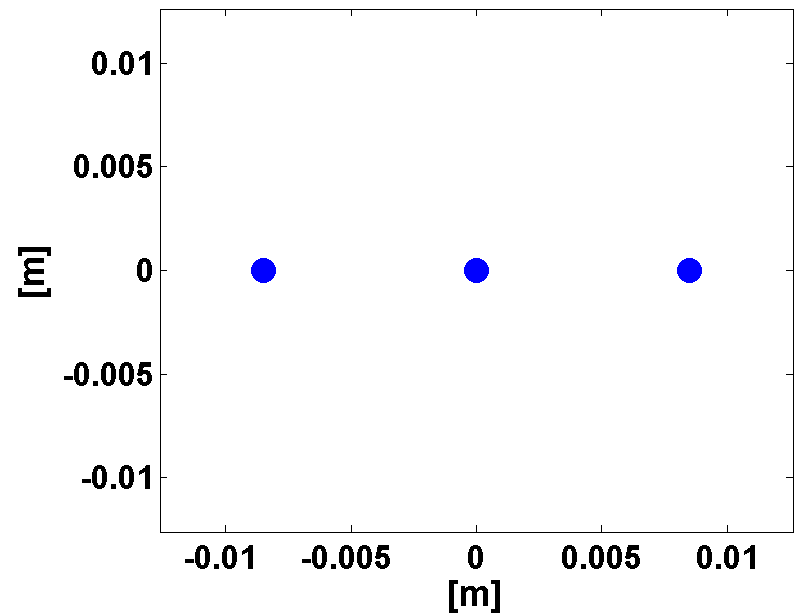
\includegraphics[width=35mm]{SecondOrderArbGeo_Linear.png}
			\label{FigLbl_SecondOrderArbGeo_Linear}}
		\quad
		\subfigure[Circular geometry]{%
			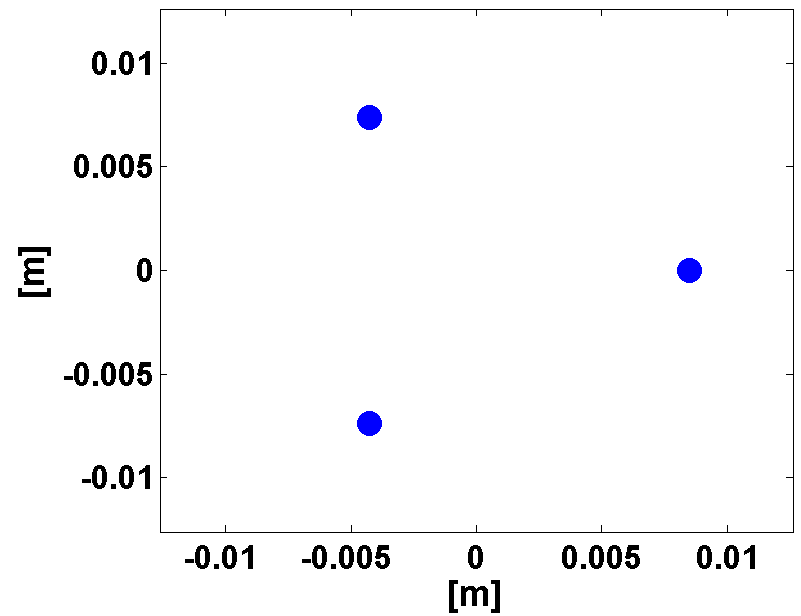
\includegraphics[width=35mm]{SecondOrderArbGeo_Circle.png}
			\label{FigLbl_SecondOrderArbGeo_Circle}}
		\subfigure[Half-circular geometry]{%
			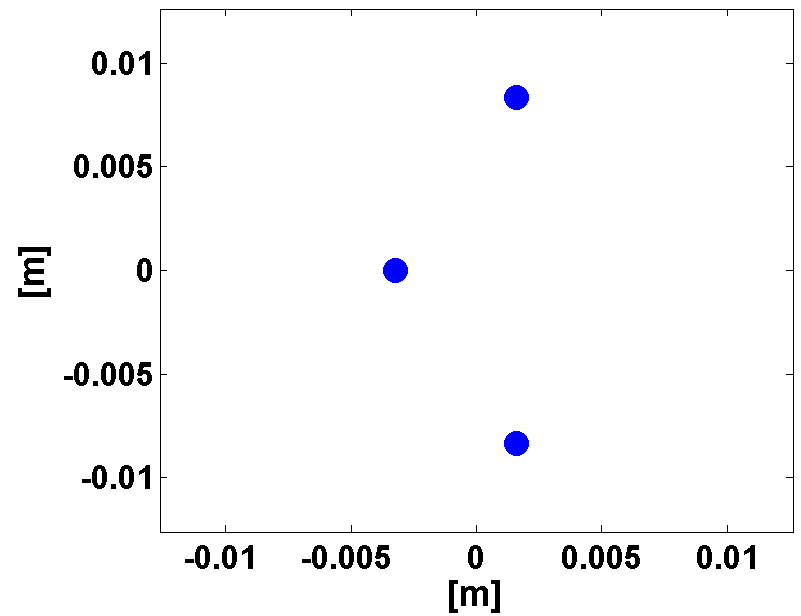
\includegraphics[width=35mm]{SecondOrderArbGeo_HalfCircle.png}
			\label{FigLbl_SecondOrderArbGeo_HalfCircle}}
		\quad
		\subfigure[Parabolic geometry]{%
			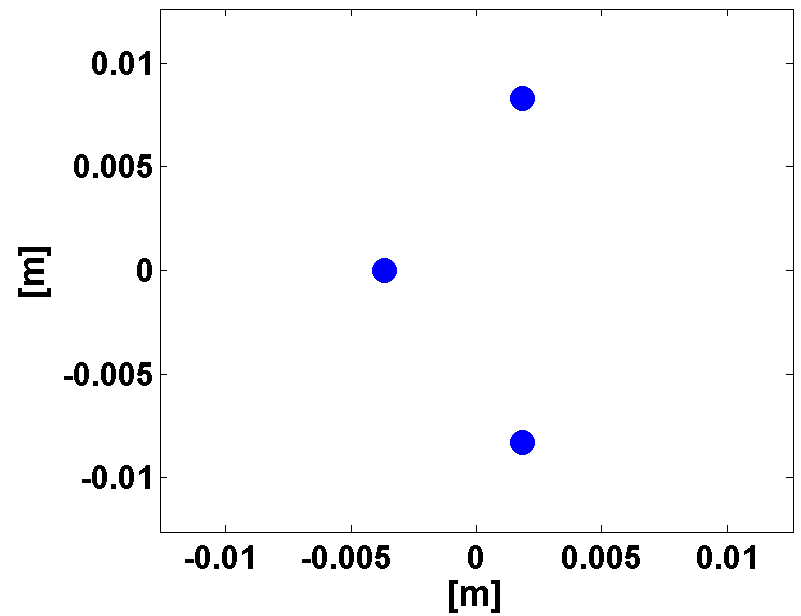
\includegraphics[width=35mm]{SecondOrderArbGeo_Parabola.png}
			\label{FigLbl_SecondOrderArbGeo_Parabola}}
		\caption{Second order geometries. basic case of M=N+1 that does not involve robustness, only the arbitrary geometry handling.}
		\label{FigLbl_SecondOrderGeometries}
	\end{figure}
	\begin{figure}[!h]
		\centering
		\subfigure[Linear geometry beampattern]{%
			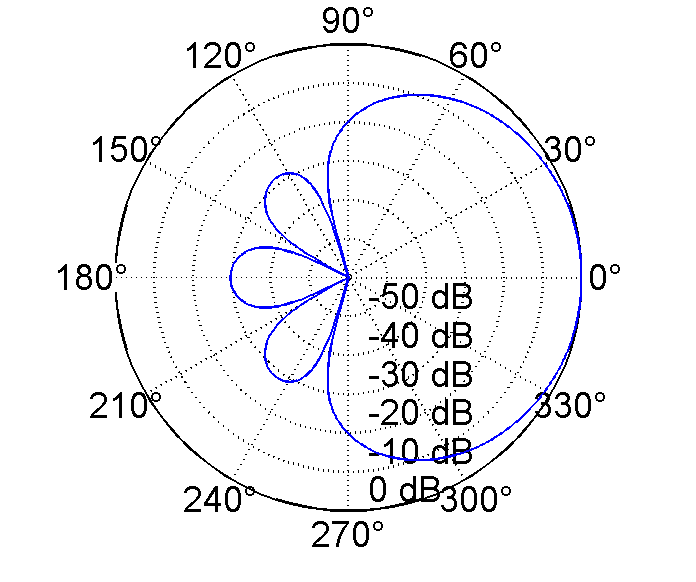
\includegraphics[width=35mm]{SecondOrderArbGeo_Linear_BP.png}
			\label{FigLbl_SecondOrderArbGeo_Linear_BP}}
		\quad
		\subfigure[Circular geometry beampattern]{%
			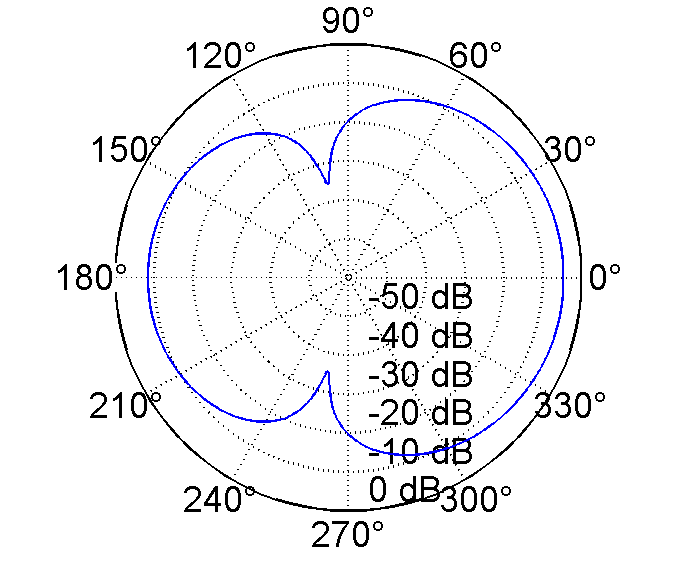
\includegraphics[width=35mm]{SecondOrderArbGeo_Circle_BP.png}
			\label{FigLbl_SecondOrderArbGeo_Circle_BP}}
		\subfigure[Half-circular geometry beampattern]{%
			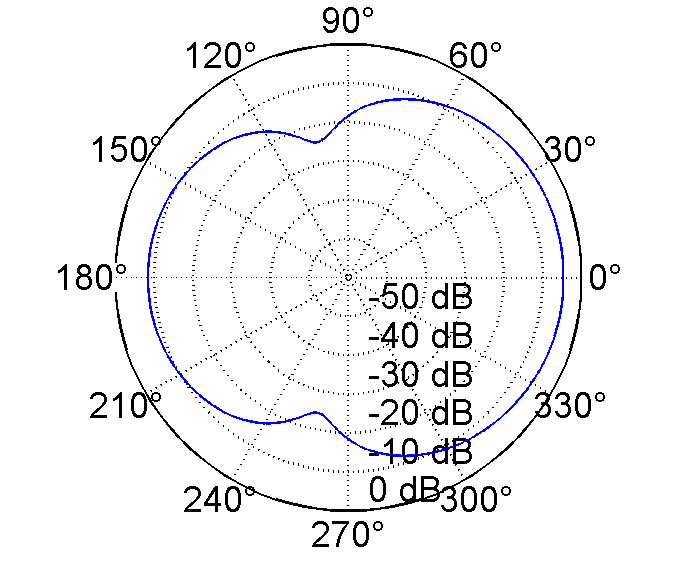
\includegraphics[width=35mm]{SecondOrderArbGeo_HalfCircle_BP.png}
			\label{FigLbl_SecondOrderArbGeo_HalfCircle_BP}}
		\quad
		\subfigure[Parabolic geometry beampattern]{%
			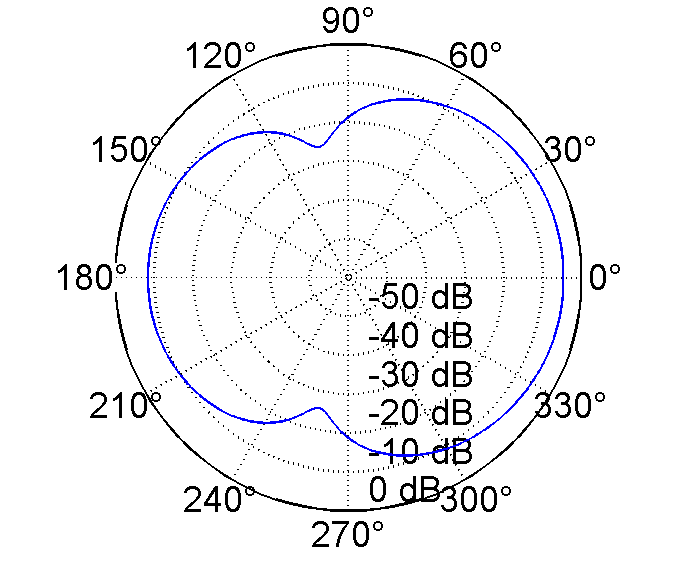
\includegraphics[width=35mm]{SecondOrderArbGeo_Parabola_BP.png}
			\label{FigLbl_SecondOrderArbGeo_Parabola_BP}}
		\caption{Second order M=N+1 beampatterns.}
		\label{FigLbl_SecondOrderGeometriesBPs}
	\end{figure}
	\begin{figure}[!h]
		\centerline{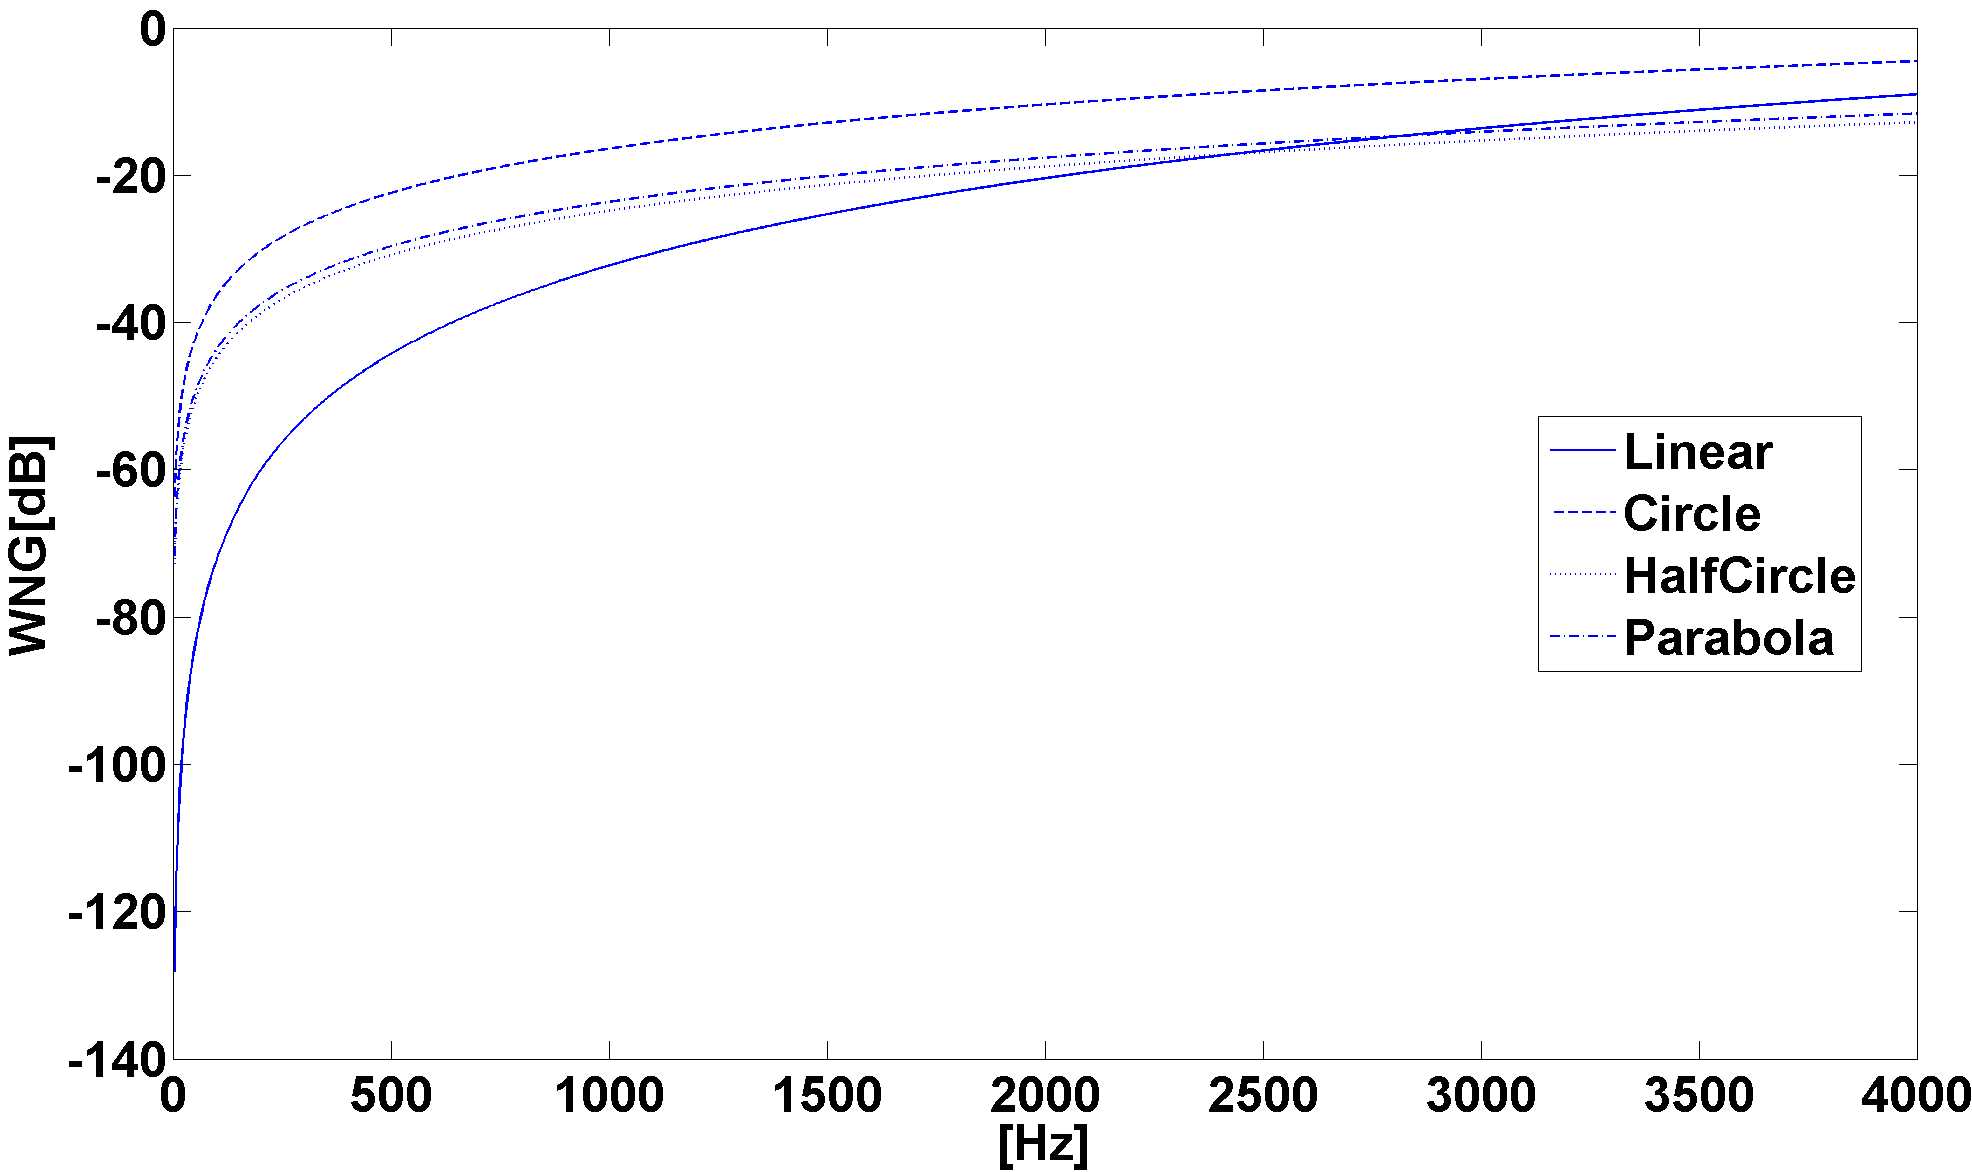
\includegraphics[width=62.5mm]{SecondOrderArbGeo_WNG.png}} \caption{{White noise gain of the regular Order+1 linear array case.}}\label{FigLbl_SecondOrderArbGeo_WNG}
	\end{figure}
	\begin{figure}[!h]
		\centerline{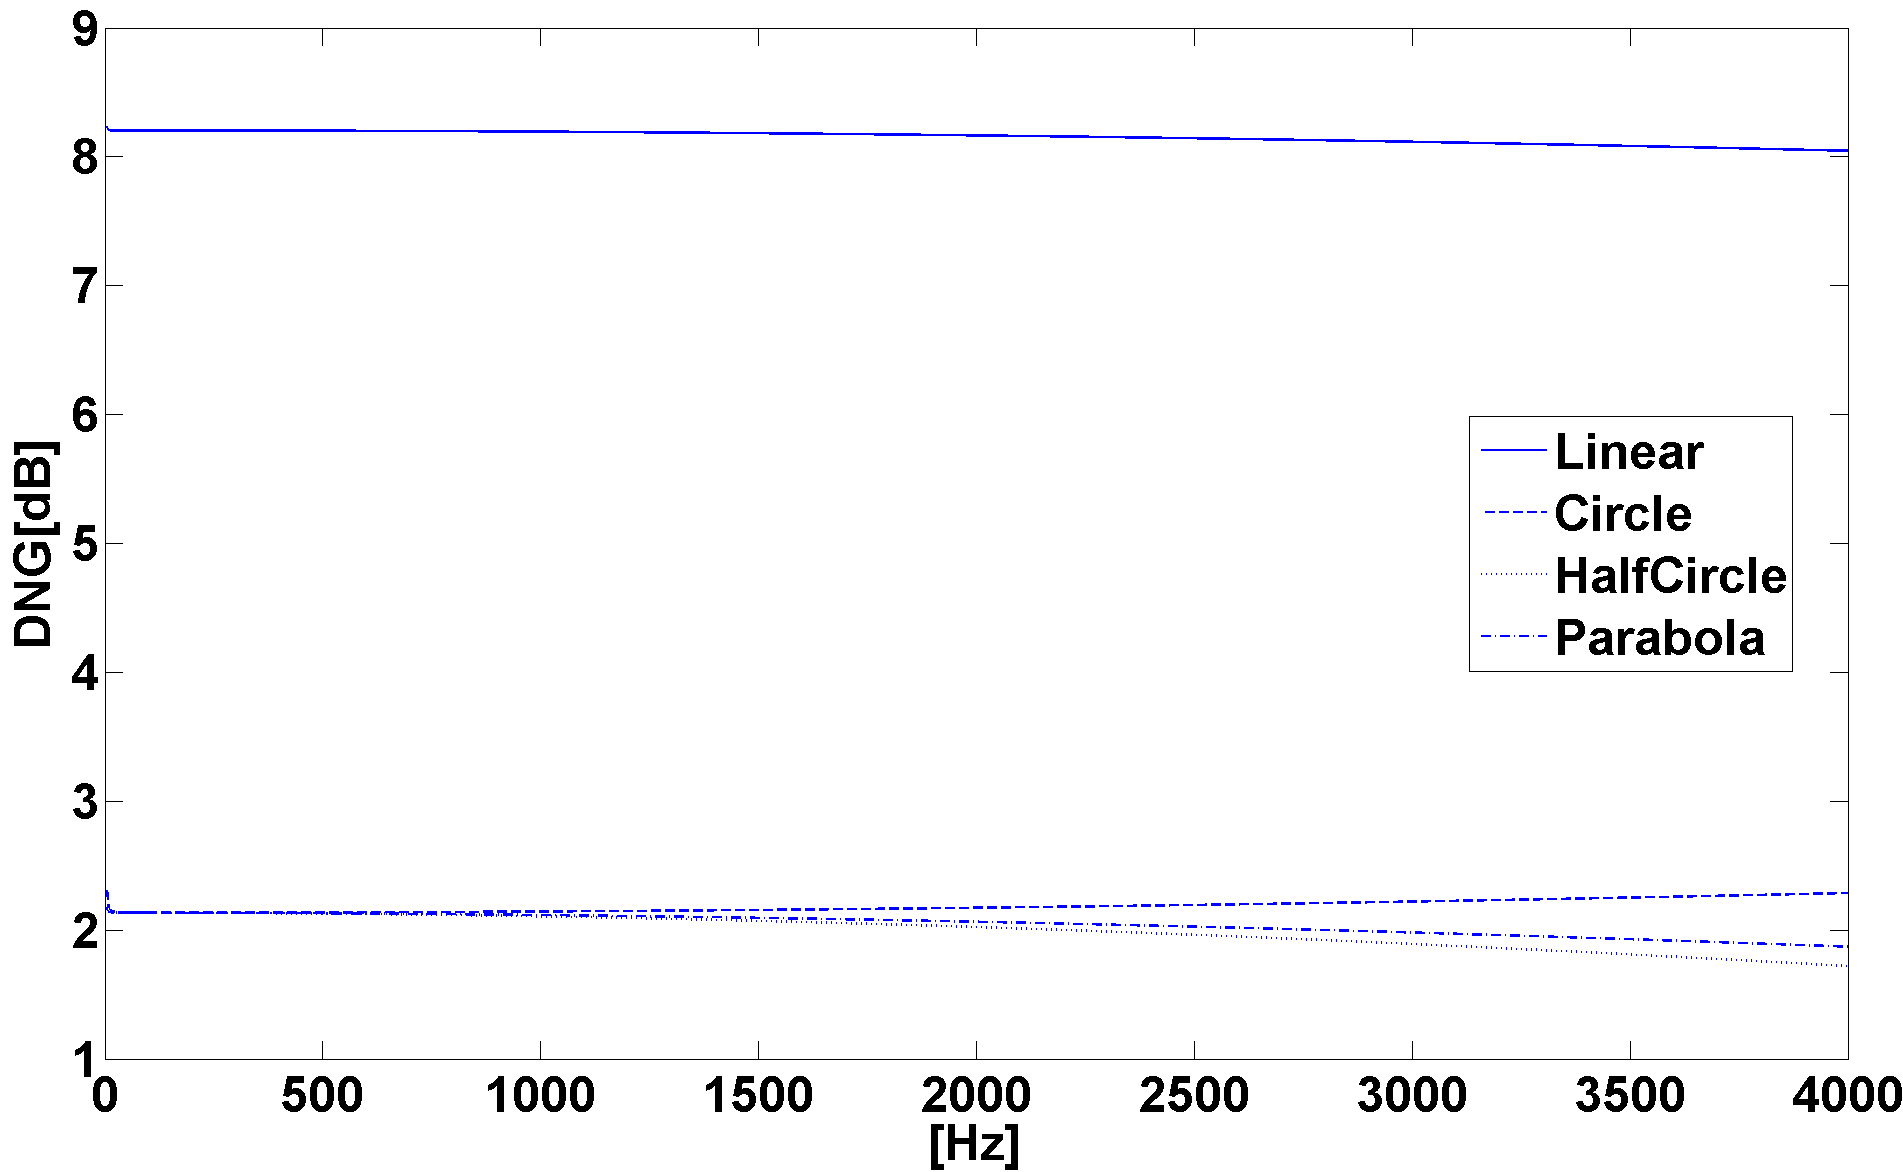
\includegraphics[width=62.5mm]{SecondOrderArbGeo_DNG.png}} \caption{{The directivity factor of the regular Order+1 linear array case. }}\label{FigLbl_SecondOrderArbGeo_DNG}
	\end{figure}
\end{center}
In figures (\ref{FigLbl_SecondOrderGeometriesBPs}) ,(\ref{FigLbl_SecondOrderArbGeo_WNG})  and (\ref{FigLbl_SecondOrderArbGeo_DNG}), we present simulation of the $ M=N+1 $ basic case. The goal of those simulations is to confirm the mathematical development and generalization of the results in \cite{sps17} to the arbitrary geometry case. We studied several different array geometries:
\begin{itemize}
	\item Linear - the basic equally spaced $ 1d $ array. $ \theta_s $ is the end-fire of the array.
	\item Circular - constant radius with equally spaced elements on the circular line. 
	\item Half-circular - constant radius with equally spaced elements on the half-circular line.
	\item Parabolic - positioning the elements according to $ y=x^2 $ while $ x $ is equally spaced in a predetermined range of values.
\end{itemize}
Already, in the basic case, we observe the geometry dependency of the \textit{beampattern}, \textit{white-noise-gain} and the \textit{directivity factor}.

\subsection{Second order robust geometries M $ > $ N+1}
\begin{center}
	\begin{figure}[!h]
		\centering
		\subfigure[Linear geometry]{%
			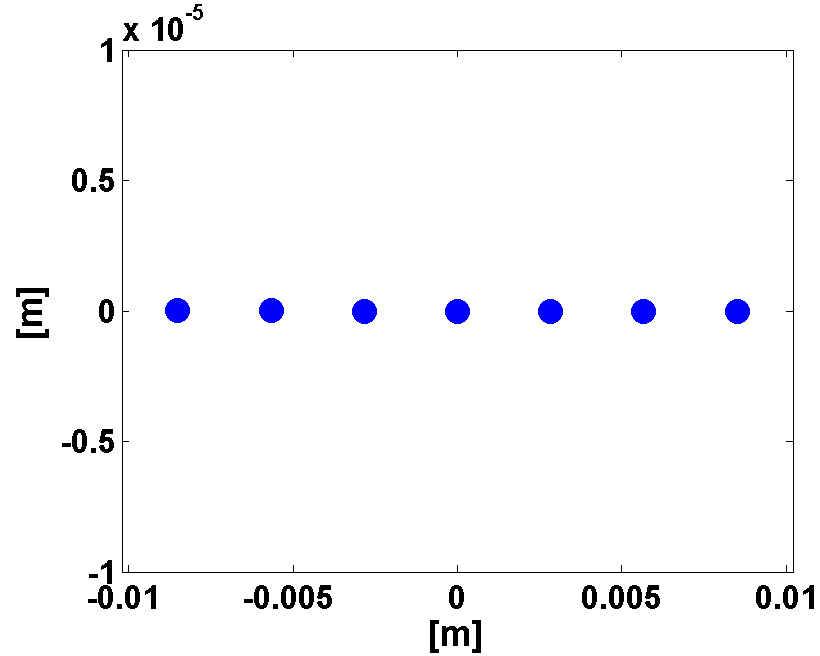
\includegraphics[width=35mm]{SecondOrderRobustArbGeo_Linear.png}
			\label{FigLbl_SecondOrderRobustArbGeo_Linear}}
		\quad
		\subfigure[Circular geometry]{%
			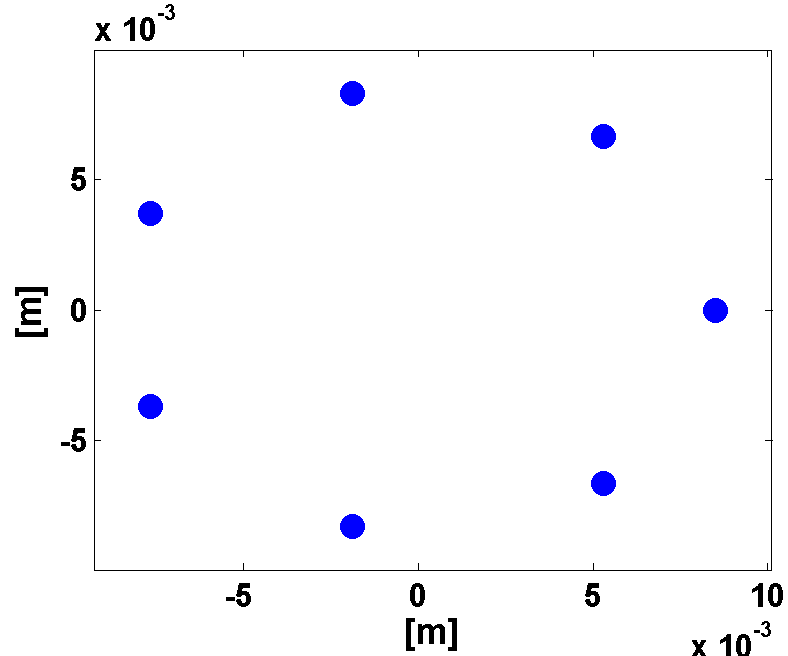
\includegraphics[width=35mm]{SecondOrderRobustArbGeo_Circle.png}
			\label{FigLbl_SecondOrderRobustArbGeo_Circle}}
		\subfigure[Half-circular geometry]{%
			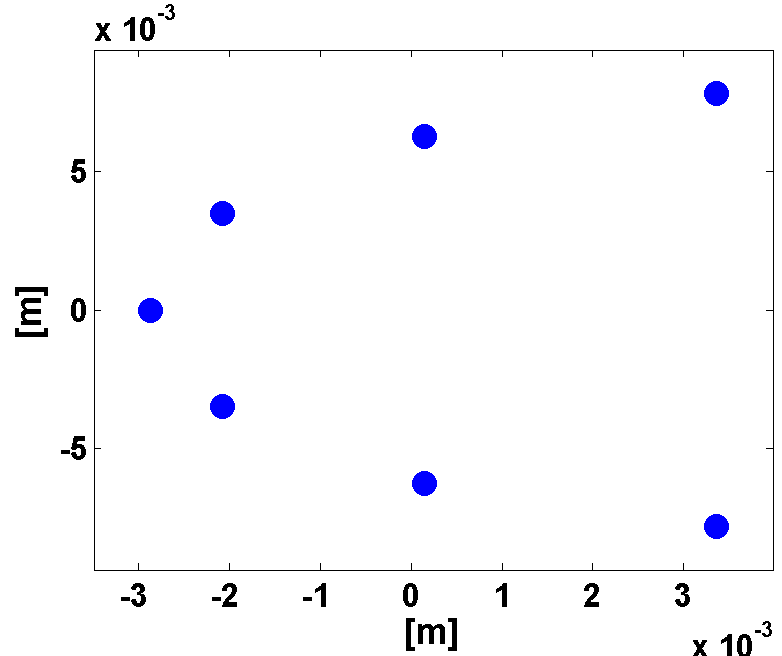
\includegraphics[width=35mm]{SecondOrderRobustArbGeo_HalfCircle.png}
			\label{FigLbl_SecondOrderRobustArbGeo_HalfCircle}}
		\quad
		\subfigure[Parabolic geometry]{%
			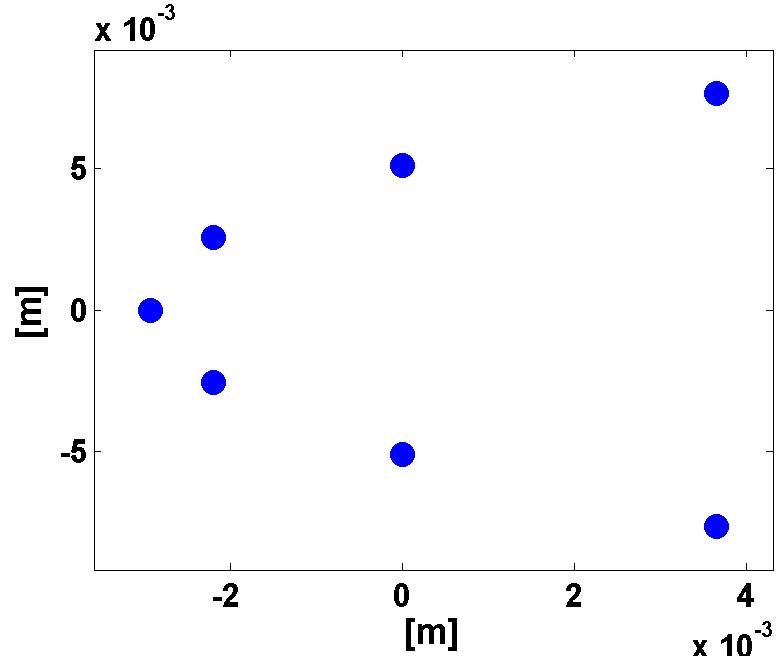
\includegraphics[width=35mm]{SecondOrderRobustArbGeo_Parabola.png}
			\label{FigLbl_SecondOrderRobustArbGeo_Parabola}}
		\caption{Second order geometries. basic case of M=N+1 that does not involve robustness, only the arbitrary geometry handling.}
		\label{FigLbl_SecondOrderGeometries}
	\end{figure}
	\begin{figure}[!h]
		\centering
		\subfigure[Linear geometry beampattern]{%
			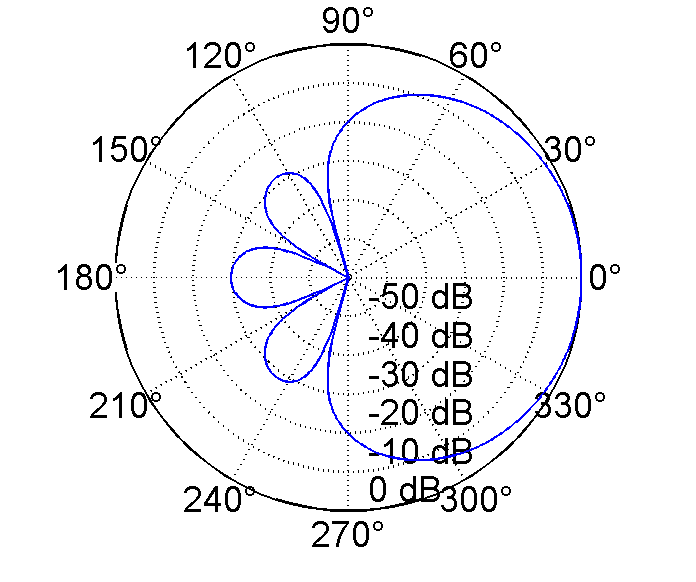
\includegraphics[width=35mm]{SecondOrderRobustArbGeo_Linear_BP.png}
			\label{FigLbl_SecondOrderRobustArbGeo_Linear_BP}}
		\quad
		\subfigure[Circular geometry beampattern]{%
			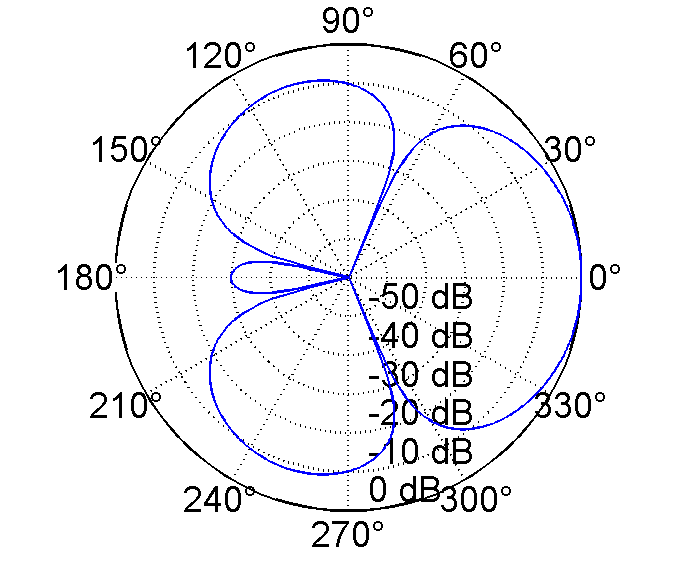
\includegraphics[width=35mm]{SecondOrderRobustArbGeo_Circle_BP.png}
			\label{FigLbl_SecondOrderRobustArbGeo_Circle_BP}}
		\subfigure[Half-circular geometry beampattern]{%
			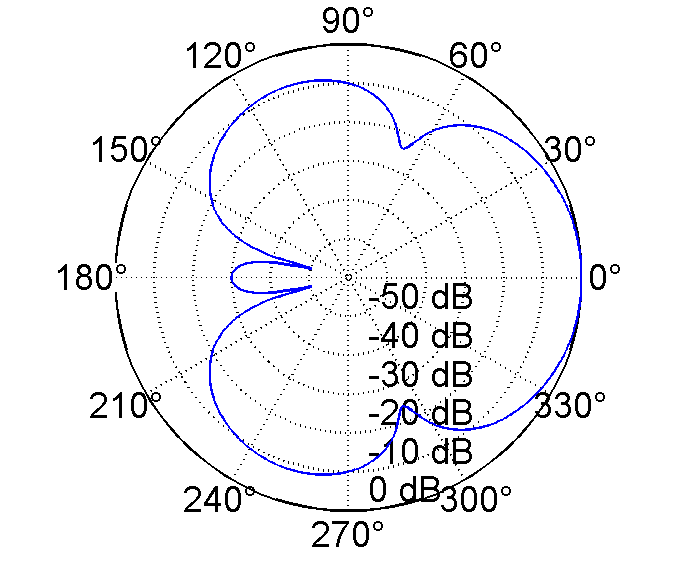
\includegraphics[width=35mm]{SecondOrderRobustArbGeo_HalfCircle_BP.png}
			\label{FigLbl_SecondOrderRobustArbGeo_HalfCircle_BP}}
		\quad
		\subfigure[Parabolic geometry beampattern]{%
			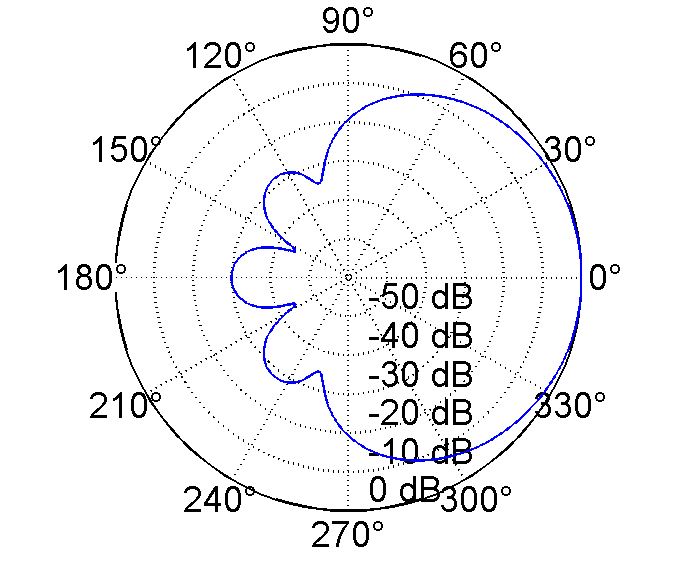
\includegraphics[width=35mm]{SecondOrderRobustArbGeo_Parabola_BP.png}
			\label{FigLbl_SecondOrderRobustArbGeo_Parabola_BP}}
		\caption{Second order M=N+1 beampatterns}
		\label{FigLbl_SecondOrderRobustGeometriesBPs}
	\end{figure}
	\begin{figure}[!h]
		\centerline{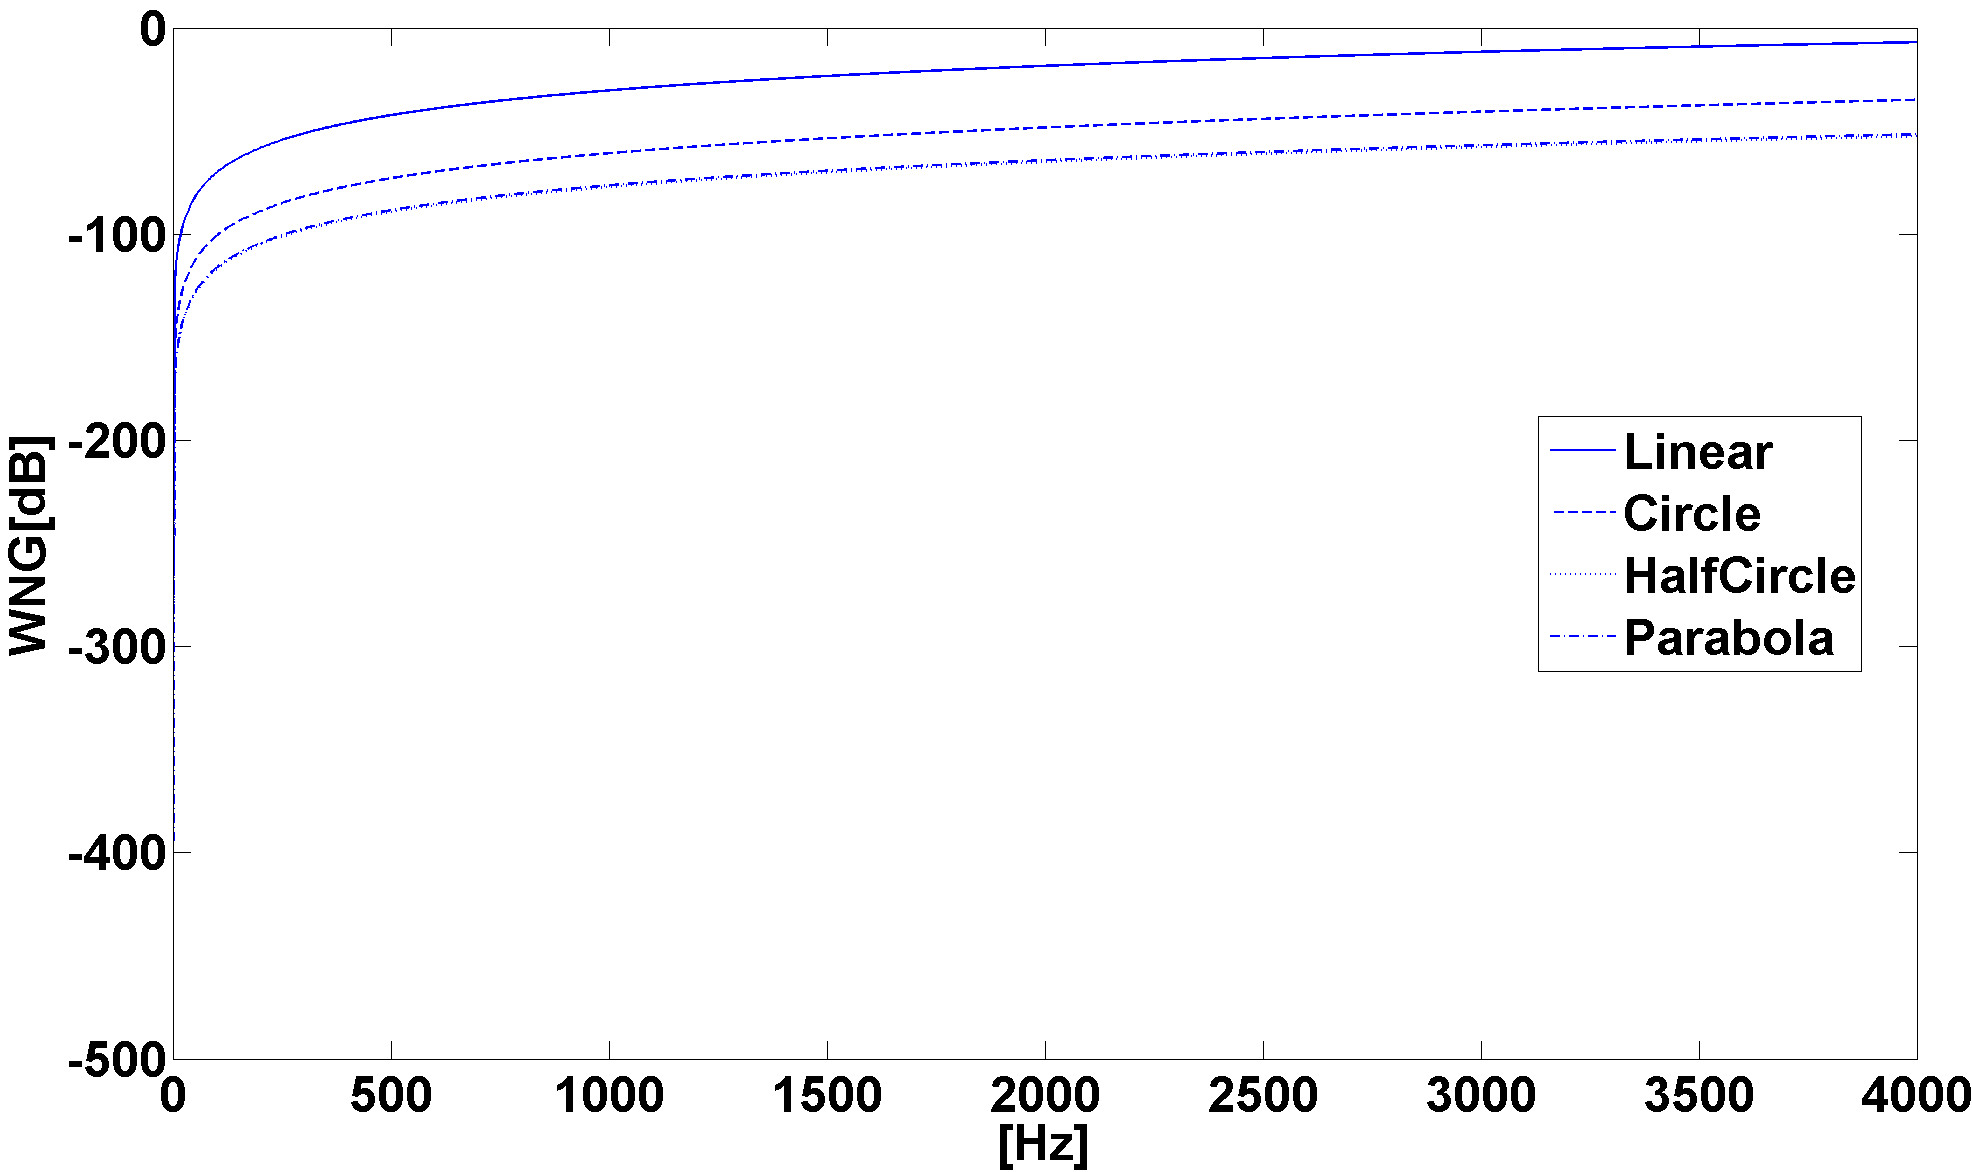
\includegraphics[width=62.5mm]{SecondOrderRobustArbGeo_WNG.png}} \caption{{White noise gain of the regular Order+1 linear array case.}}\label{FigLbl_SecondOrderRobustArbGeo_WNG}
	\end{figure}
	\begin{figure}[!h]
		\centerline{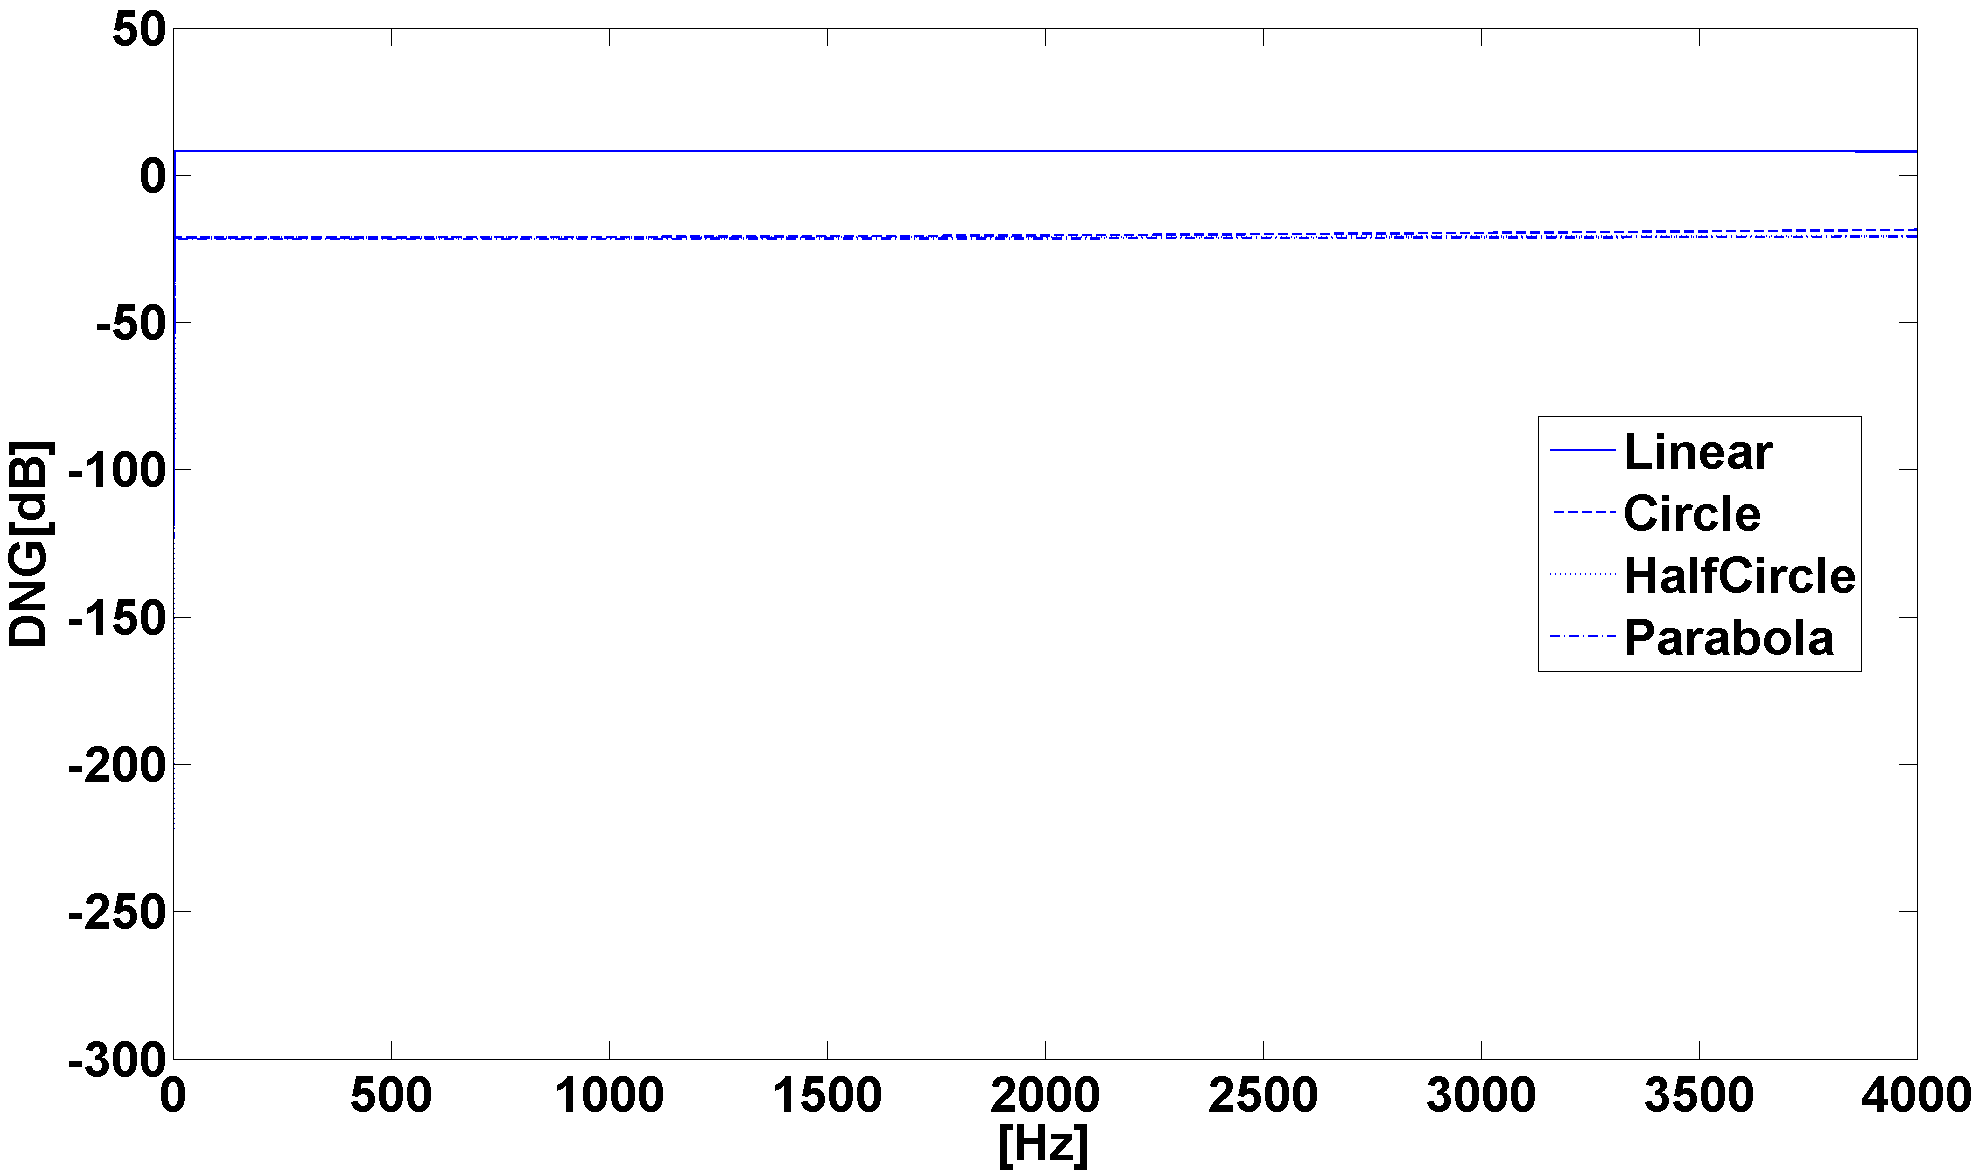
\includegraphics[width=62.5mm]{SecondOrderRobustArbGeo_DNG.png}} \caption{{The directivity factor of the regular Order+1 linear array case.}}\label{FigLbl_SecondOrderRobustArbGeo_DNG}
	\end{figure}
\end{center}
In figures (\ref{FigLbl_SecondOrderRobustGeometriesBPs}) ,(\ref{FigLbl_SecondOrderRobustArbGeo_WNG})  and (\ref{FigLbl_SecondOrderRobustArbGeo_DNG}), we add the robustness layer that was developed in \cite{sps17} and generalized in this paper to the arbitrary geometry case. We simulated again second order arrays but with 5 elements, using the two additional microphones for robustness. A very interesting and surprising result is that the robustness to white noise which is significantly improved in the linear geometry, is actually worsened in the non-linear geometries. Heuristically comparing the two cases, one can easily observe that if a specific geometry better performed (in terms of \textit{white-noise gain}, \text{directivity factor} or both) another geometry in the $ M=N+1 $ case, it doesn't guaranty that it would also outperform in the robust case.   
\section{Conclusions}
In this paper, the main goal was to achieve a generalized method of constructing a frequency-invariant beam former with an arbitrary 2D geometry arrays. In the presented simulations, one can see the differences between the various array geometries. We also demonstrated how concepts such as the robustness of arrays when adding more elements than the $ Order+1 $ is not trivial when leaving the linear array case. Many other surprising results lie in the final simulation but more work should be done to achieve sufficient explanations. Further work could be on generalizing the system to a $ 3D $ arrays, adding the elevation angle to the equations, learning the impact of array shape on the final outcome and much more.
%% References should be produced using the bibtex program from suitable
%% BiBTeX files (here: strings, refs, manuals). The IEEEbib.bst bibliography
%% style file from IEEE produces unsorted bibliography list.
%% -------------------------------------------------------------------------
\bibliographystyle{IEEEbib}
\bibliography{refs}
%
\end{document}
